\chapter{Implementacija i korisničko sučelje}


\section{Korištene tehnologije i alati}


\hspace{0.67cm}Komunikacija u timu odvijala se putem aplikacija \underline{WhatsApp}\footnote{\url{https://www.whatsapp.com/}} i \underline{Discord}\footnote{\url{https://discord.com/}}.
Kao sustav za upravljanje izvornim kodom korišten je \underline{Git}\footnote{\url{https://git-scm.com/}}, distribuirani sustav kontrole verzija koji prati promjene u bilo kojem skupu datoteka. Udaljeni repozitorij projekta je dostupan na web platformi \underline{GitLab}\footnote{\url{https://about.gitlab.com/}}.

UML dijagrami su napravljeni u \underline{Visual Paradigm Online}\footnote{\url{https://www.visual-paradigm.com/}}, besplatnom alatu za crtanje.

Pri oblikovanju aplikacije za \textit{backend}  je korišten radni okvir \underline{Spring Boot}\footnote{\url{https://spring.io/projects/spring-boot/}} i jezik \underline{Java}\footnote{\url{https://www.java.com/en/}}. Spring Boot je otvoreni Java radni okvir namijenjen pojednostavljenoj izgradnji samostalnih, produkcijski orijentiranih Spring aplikacija. Pruža optimiziranu platformu za razvoj Java aplikacija s naglaskom na konvenciju umjesto konfiguracije, omogućavajući programerima brzo postavljanje i razvoj robusnih, skalabilnih i efikasnih aplikacija. Spring Boot dolazi s ugrađenim značajkama poput automatske konfiguracije, podrške za ugrađeni web poslužitelj i postavkama spremnim za produkcijsko okruženje. Java je objektno orijentirani i platformski neovisan programski jezik. Kod napisan u Javi može izvoditi na bilo kojem uređaju ili platformi s Java Virtual Machine (JVM). Java je poznata po svojoj prenosivosti, snažnoj podršci zajednice i obilnim bibliotekama, što je čini popularnim izborom za izgradnju različitih vrsta aplikacija.




Za implementaciju \textit{frontenda} koristili smo razvojno okruženje \underline{React}\footnote{\url{https://react.dev/}} i jezik \underline{JavaScript}\footnote{\url{https://www.javascript.com/}}. React je otvorena JavaScript biblioteka za izgradnju korisničkih sučelja. Omogućuje stvaranje ponovno upotrebljivih komponenti korisničkog sučelja, upravljanje njihovim vlastitim stanjem i učinkovito ažuriranje korisničkog sučelja putem virtualnog DOM-a. React slijedi jednosmjerni tok podataka, koristi JSX za sintaksu komponenata i široko se koristi zbog modularnosti i optimizacija performansi.
JavaScript je svestrani i objektno orijentirani jezik, uglavnom korišten za stvaranje dinamičnog i interaktivnog sadržaja na web stranicama. Podržava asinkrono programiranje i radi na različitim platformama, što ga čini ključnom tehnologijom u web razvoju. Osim u preglednicima, proširuje se i na druge domene, uključujući i izradu mobilnih aplikacija. 

\underline{LaTeX}\footnote{\url{https://www.latex-project.org/}} je sustav za stvaranje visokokvalitetnih dokumenata, posebno u znanstvenim i akademskim kontekstima. Koristi označavanje teksta pomoću naredbi kako bi se definirala struktura dokumenta i formatiranje. Korisnici pišu dokumente u običnom tekstu s ekstenzijom .tex i koriste LaTeX compiler za generiranje formatiranih izlaza, često u PDF formatu.


\eject 


\section{Ispitivanje programskog rješenja}

\textbf{\textit{dio 2. revizije}}\\

\textit{U ovom poglavlju je potrebno opisati provedbu ispitivanja implementiranih funkcionalnosti na razini komponenti i na razini cijelog sustava s prikazom odabranih ispitnih slučajeva. Studenti trebaju ispitati temeljnu funkcionalnost i rubne uvjete.}


\subsection{Ispitivanje komponenti}

Ispitivanje komponenti provjerava ispravnost djelovanja pojedinih dijelova programa koji su mogući za odvojeno ispitivanje, poput pojedinačnih funkcija ili metoda unutar objekta.

Ispitivanje komponenti za CreateKorisnikTest fokusira se na verifikaciju funkcionalnosti klase KorisnikService prilikom stvaranja novog korisnika. Testiraju se različiti scenariji, uključujući prepoznavanje već postojećeg emaila ili korisničkog imena te obrada null vrijednosti slike.

\begin{figure}[H]
	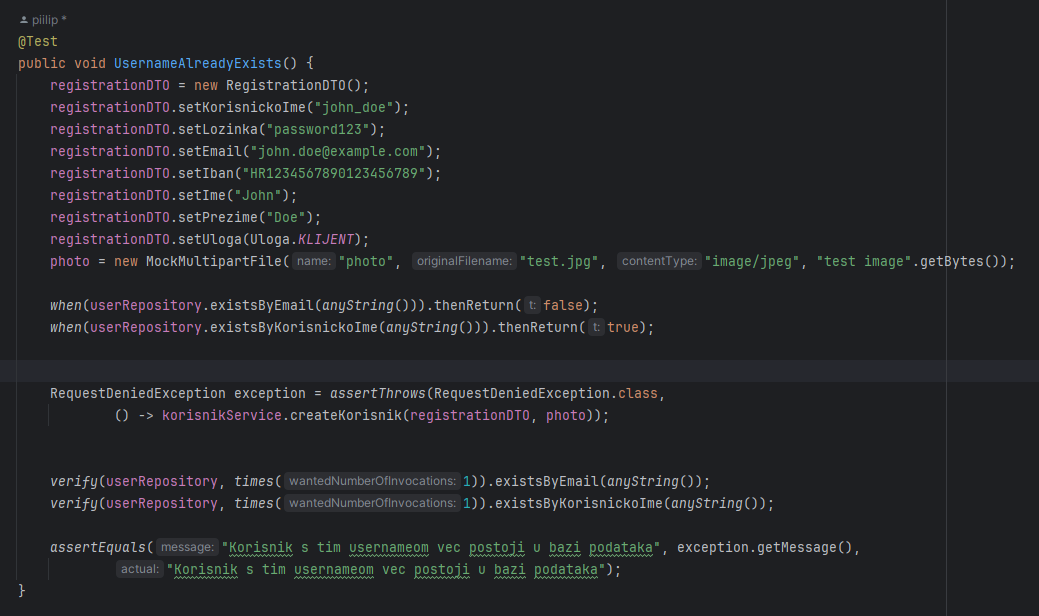
\includegraphics[width=\textwidth]{slike/username.png} %veličina slike u odnosu na originalnu datoteku i pozicija slike
	\centering
	\caption{1. ispitni slučaj za CreateKorisnikTest}
	\label{fig:dijagramstanja}
\end{figure}

\begin{figure}[H]
	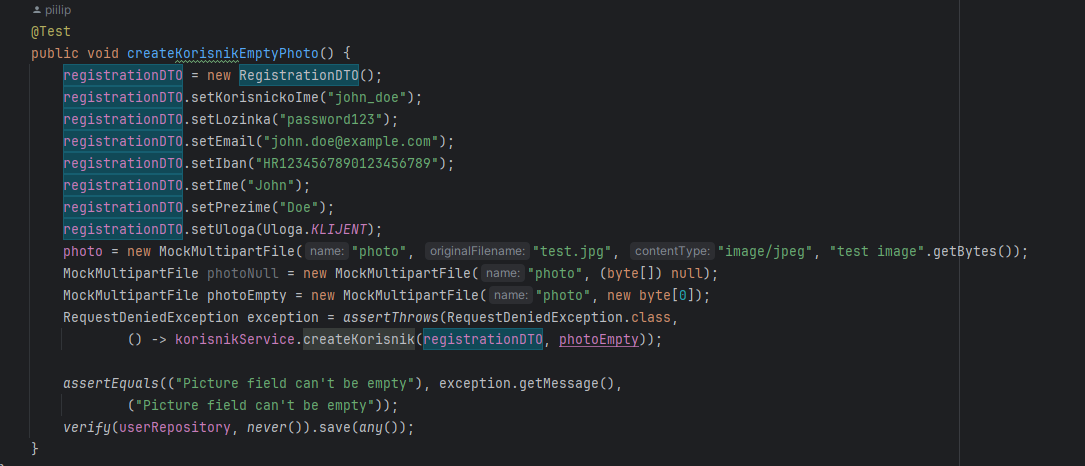
\includegraphics[width=\textwidth]{slike/korisnikslika.png} %veličina slike u odnosu na originalnu datoteku i pozicija slike
	\centering
	\caption{2. ispitni slučaj za CreateKorisnikTest}
	\label{fig:dijagramstanja}
\end{figure}

\begin{figure}[H]
	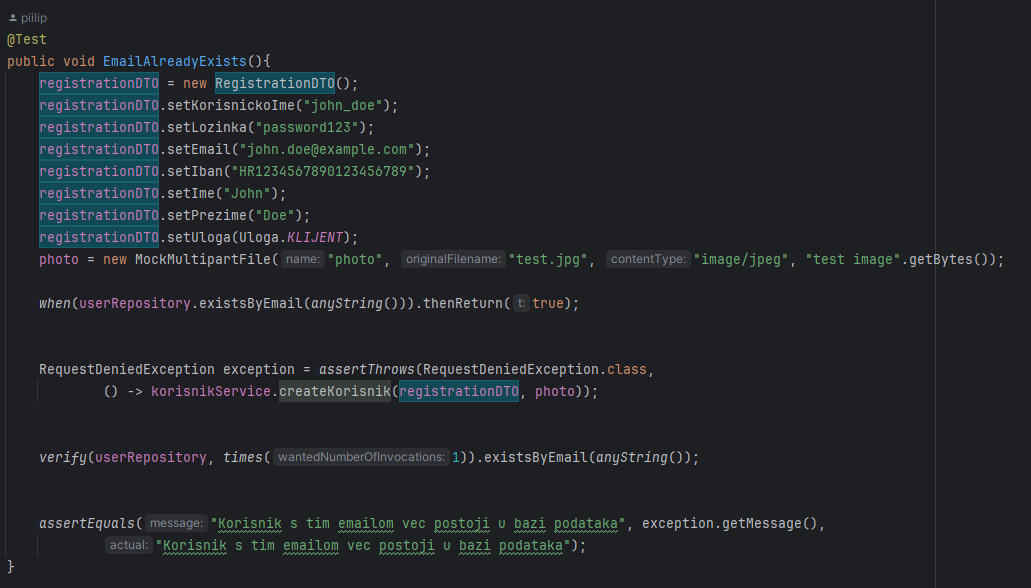
\includegraphics[width=\textwidth]{slike/email.png} %veličina slike u odnosu na originalnu datoteku i pozicija slike
	\centering
	\caption{3. ispitni slučaj za CreateKorisnikTest}
	\label{fig:dijagramstanja}
\end{figure}

Ispitivanje komponenti za UpdateKorisnikTest usmjereno je na verifikaciju funkcionalnosti metode updateKorisnik unutar klase KorisnikService. Testiraju se scenariji ažuriranja korisničkih podataka, uključujući promjenu korisničkog imena, imena, lozinke i slike.

\begin{figure}[H]
	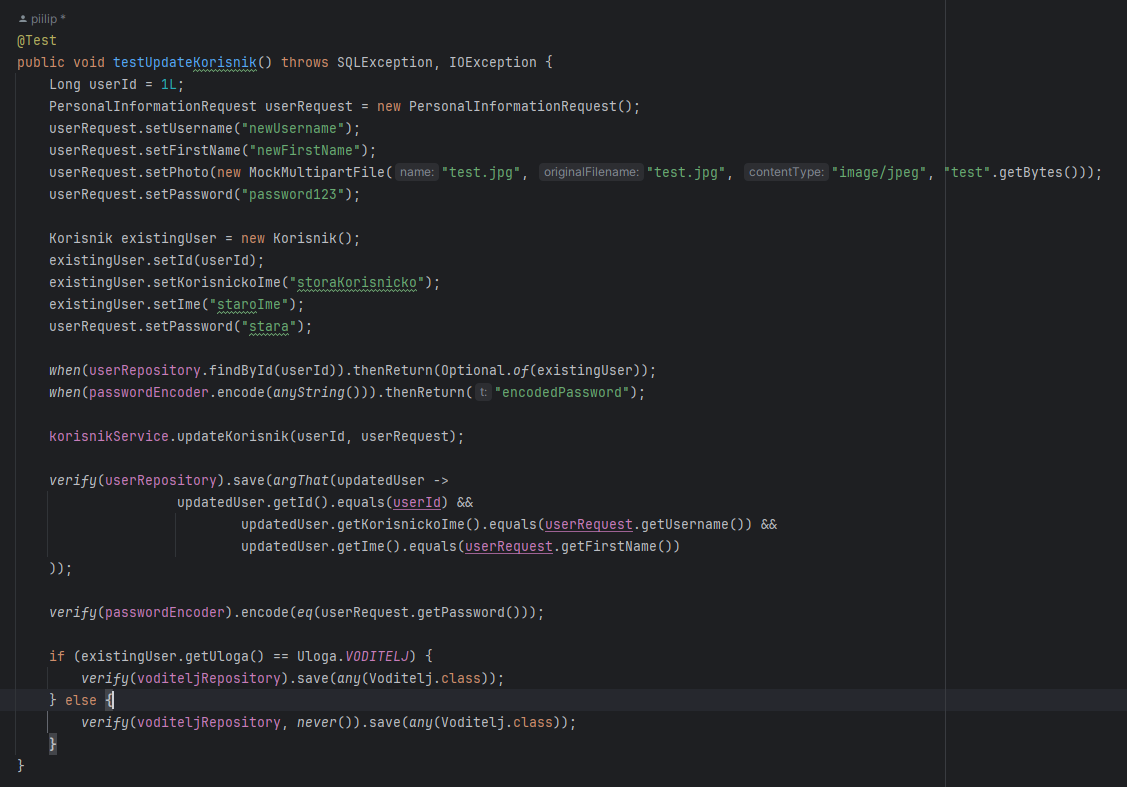
\includegraphics[width=\textwidth]{slike/testupdatekorisnik.png} %veličina slike u odnosu na originalnu datoteku i pozicija slike
	\centering
	\caption{1. ispitni slučaj za UpdateKorisnikTest}
	\label{fig:dijagramstanja}
\end{figure}


Ispitivanje komponenti za ParkingServiceTest usmjereno je na verifikaciju funkcionalnosti klase ParkingService. Fokusirano je na ispravno označavanje parkirnih mjesta kao rezervirana i ponašanje sustava u različitim scenarijima(verifikacija ispravnosti označavanja parkirnih mjesta kao rezervirana, provjera ponašanja sustava u slučaju nepostojećeg parkirališta, verifikacija ponašanja sustava kada je parkirno mjesto već označeno i testiranje ispravnosti dobivanja indeksa najmanje udaljenosti).

\begin{figure}[H]
	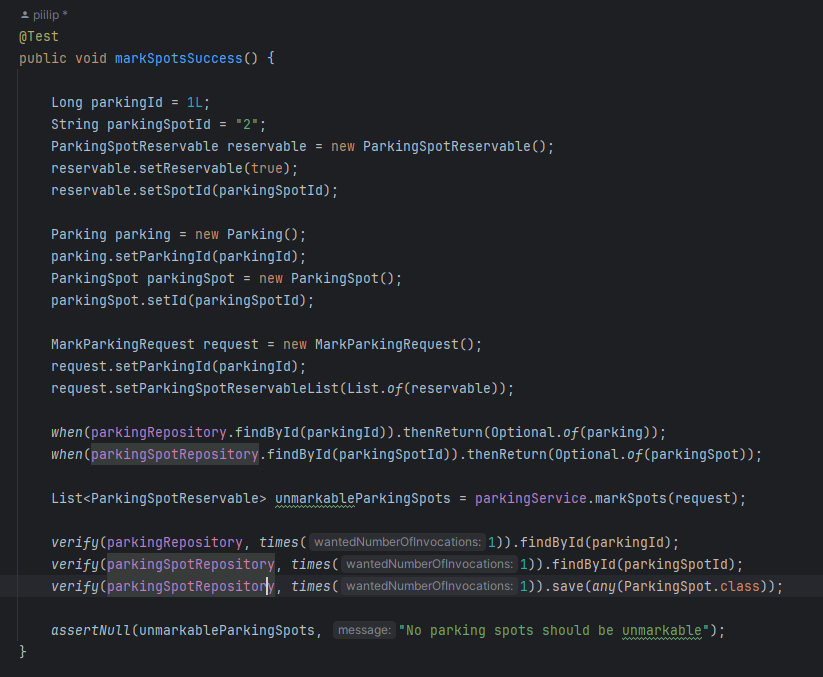
\includegraphics[width=\textwidth]{slike/markspotsuccess.png} %veličina slike u odnosu na originalnu datoteku i pozicija slike
	\centering
	\caption{1. ispitni slučaj za ParkingServiceTest}
	\label{fig:dijagramstanja}
\end{figure}


\begin{figure}[H]
	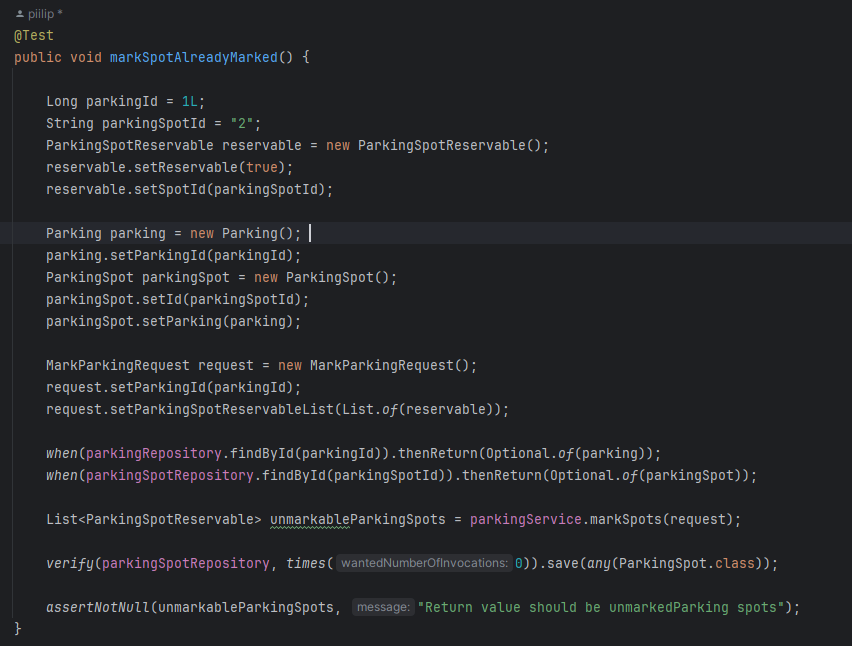
\includegraphics[width=\textwidth]{slike/markspotmarked.png} %veličina slike u odnosu na originalnu datoteku i pozicija slike
	\centering
	\caption{2. ispitni slučaj za ParkingServiceTest}
	\label{fig:dijagramstanja}
\end{figure}

\begin{figure}[H]
	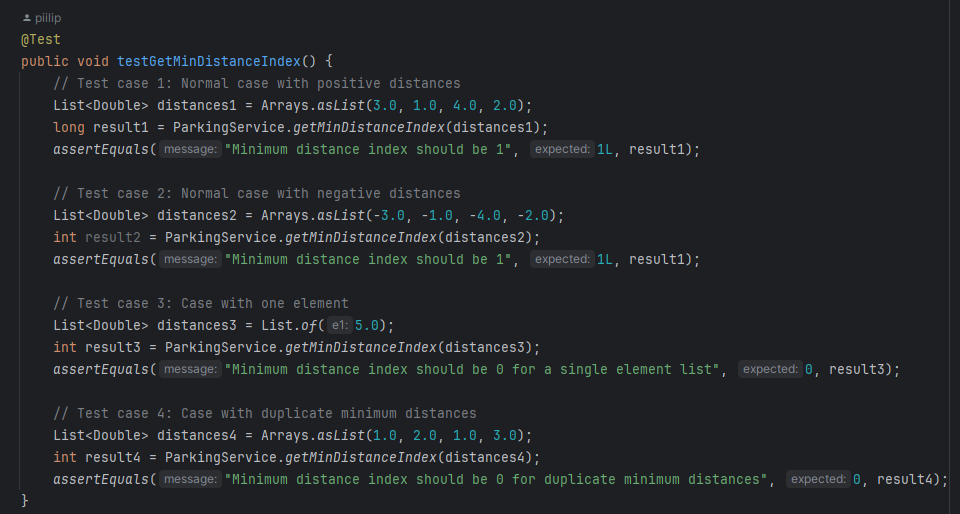
\includegraphics[width=\textwidth]{slike/testmindistance.png} %veličina slike u odnosu na originalnu datoteku i pozicija slike
	\centering
	\caption{3. ispitni slučaj za ParkingServiceTest}
	\label{fig:dijagramstanja}
\end{figure}

\begin{figure}[H]
	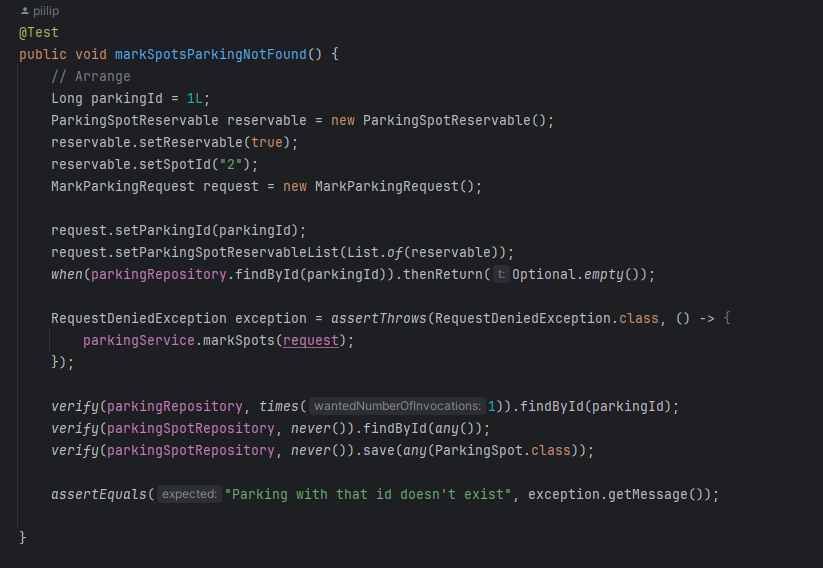
\includegraphics[width=\textwidth]{slike/markspotparking.png} %veličina slike u odnosu na originalnu datoteku i pozicija slike
	\centering
	\caption{4. ispitni slučaj za ParkingServiceTest}
	\label{fig:dijagramstanja}
\end{figure}

\subsection{Ispitivanje sustava}

\textit{Potrebno je provesti i opisati ispitivanje sustava koristeći radni okvir Selenium\footnote{\url{https://www.seleniumhq.org/}}. Razraditi \textbf{minimalno 4 ispitna slučaja} u kojima će se ispitati redovni slučajevi, rubni uvjeti te poziv funkcionalnosti koja nije implementirana/izaziva pogrešku kako bi se vidjelo na koji način sustav reagira kada nešto nije u potpunosti ostvareno. Ispitni slučaj se treba sastojati od ulaza (npr. korisničko ime i lozinka), očekivanog izlaza ili rezultata, koraka ispitivanja i dobivenog izlaza ili rezultata.\\ }

\textit{Izradu ispitnih slučajeva pomoću radnog okvira Selenium moguće je provesti pomoću jednog od sljedeća dva alata:}
\begin{itemize}
	\item \textit{dodatak za preglednik \textbf{Selenium IDE} - snimanje korisnikovih akcija radi automatskog ponavljanja ispita	}
	\item \textit{\textbf{Selenium WebDriver} - podrška za pisanje ispita u jezicima Java, C\#, PHP koristeći posebno programsko sučelje.}
\end{itemize}
\textit{Detalji o korištenju alata Selenium bit će prikazani na posebnom predavanju tijekom semestra.}

\eject 


\section{Dijagram razmještaja}


UML-dijagrami razmještaja (engl. deployment diagrams) su takoder vrsta strukturnih UML-dijagrama koji prikazuju fizičku arhitekturu i konfiguraciju razmještaja programskog sustava. Oni ilustriraju raspodjelu programskih komponenti, izvršnih datoteka i knjižnica na sklopovske čvorove ili virtualna izvršna okruženja.
Na poslužiteljskom računalu nalaze se Web poslužitelj i poslužitelj baze podataka. Korisnik do web aplikacije dolazi preko web preglednika pri čemu mobilna aplikacija komunicira s poslužiteljem pomoću protokola HTTP. Osim s korisnikom, web poslužitelj komunicira i s OSRM pomoću protokola HTTP.

\vspace{5cm}

\begin{figure}[H]
	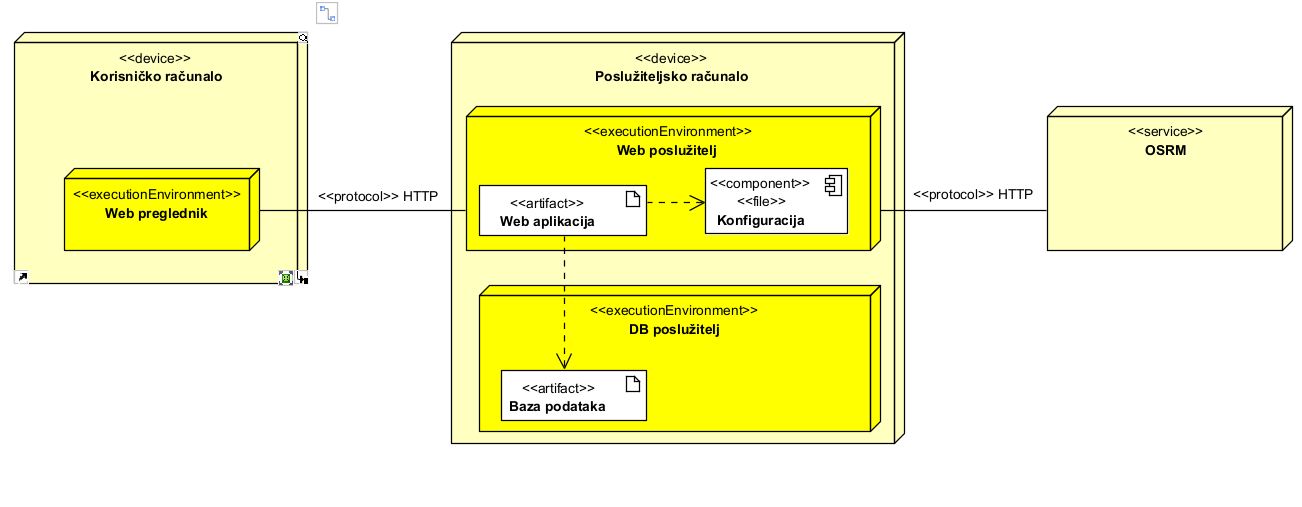
\includegraphics[width=\textwidth]{slike/dijagram_razmjestaja.png} %veličina slike u odnosu na originalnu datoteku i pozicija slike
	\centering
	\caption{Dijagram razmještaja}
	\label{fig:dijagramaktivnosti}
\end{figure}
\eject 

\section{Upute za puštanje u pogon}

\textbf{\textit{dio 2. revizije}}\\

\textit{U ovom poglavlju potrebno je dati upute za puštanje u pogon (engl. deployment) ostvarene aplikacije. Na primjer, za web aplikacije, opisati postupak kojim se od izvornog kôda dolazi do potpuno postavljene baze podataka i poslužitelja koji odgovara na upite korisnika. Za mobilnu aplikaciju, postupak kojim se aplikacija izgradi, te postavi na neku od trgovina. Za stolnu (engl. desktop) aplikaciju, postupak kojim se aplikacija instalira na računalo. Ukoliko mobilne i stolne aplikacije komuniciraju s poslužiteljem i/ili bazom podataka, opisati i postupak njihovog postavljanja. Pri izradi uputa preporučuje se \textbf{naglasiti korake instalacije uporabom natuknica} te koristiti što je više moguće \textbf{slike ekrana} (engl. screenshots) kako bi upute bile jasne i jednostavne za slijediti.}


\textit{Dovršenu aplikaciju potrebno je pokrenuti na javno dostupnom poslužitelju. Studentima se preporuča korištenje neke od sljedećih besplatnih usluga: \href{https://aws.amazon.com/}{Amazon AWS}, \href{https://azure.microsoft.com/en-us/}{Microsoft Azure} ili \href{https://www.heroku.com/}{Heroku}. Mobilne aplikacije trebaju biti objavljene na F-Droid, Google Play ili Amazon App trgovini.}


\eject 